\section{RHUL Keysight pulse generator}
 \begin{itemize}
 	\item \cmd{\quote{Utility} \ira \quote{I/O Interface} \ira \quote{LAN} \ira Set IP, DNS and Subnet, the last two as shwon in \quote{Network connection details}};
 	\item \cmd{Type in the IP given to the device in a web browser and get the \quote{VISA TCPIP Connect String}};
 	\item \cmd{Use this string as the input argument to \quote{VISA OPEN} and you can send commands};
 	\item \textbf{Chapter 3} of the manual has the remote commands that you can send;
 	\item It has an refference out port from the back. \cmd{\quote{Utility}\ira\quote{Refferenfce clock}} allows you to choose it as the internal source clock. \red{Now, all the generated pulses will be in sync with this clock \ira it can be used as a refference clock for other components too.}
 \end{itemize}

	\begin{figure}
		\centering
		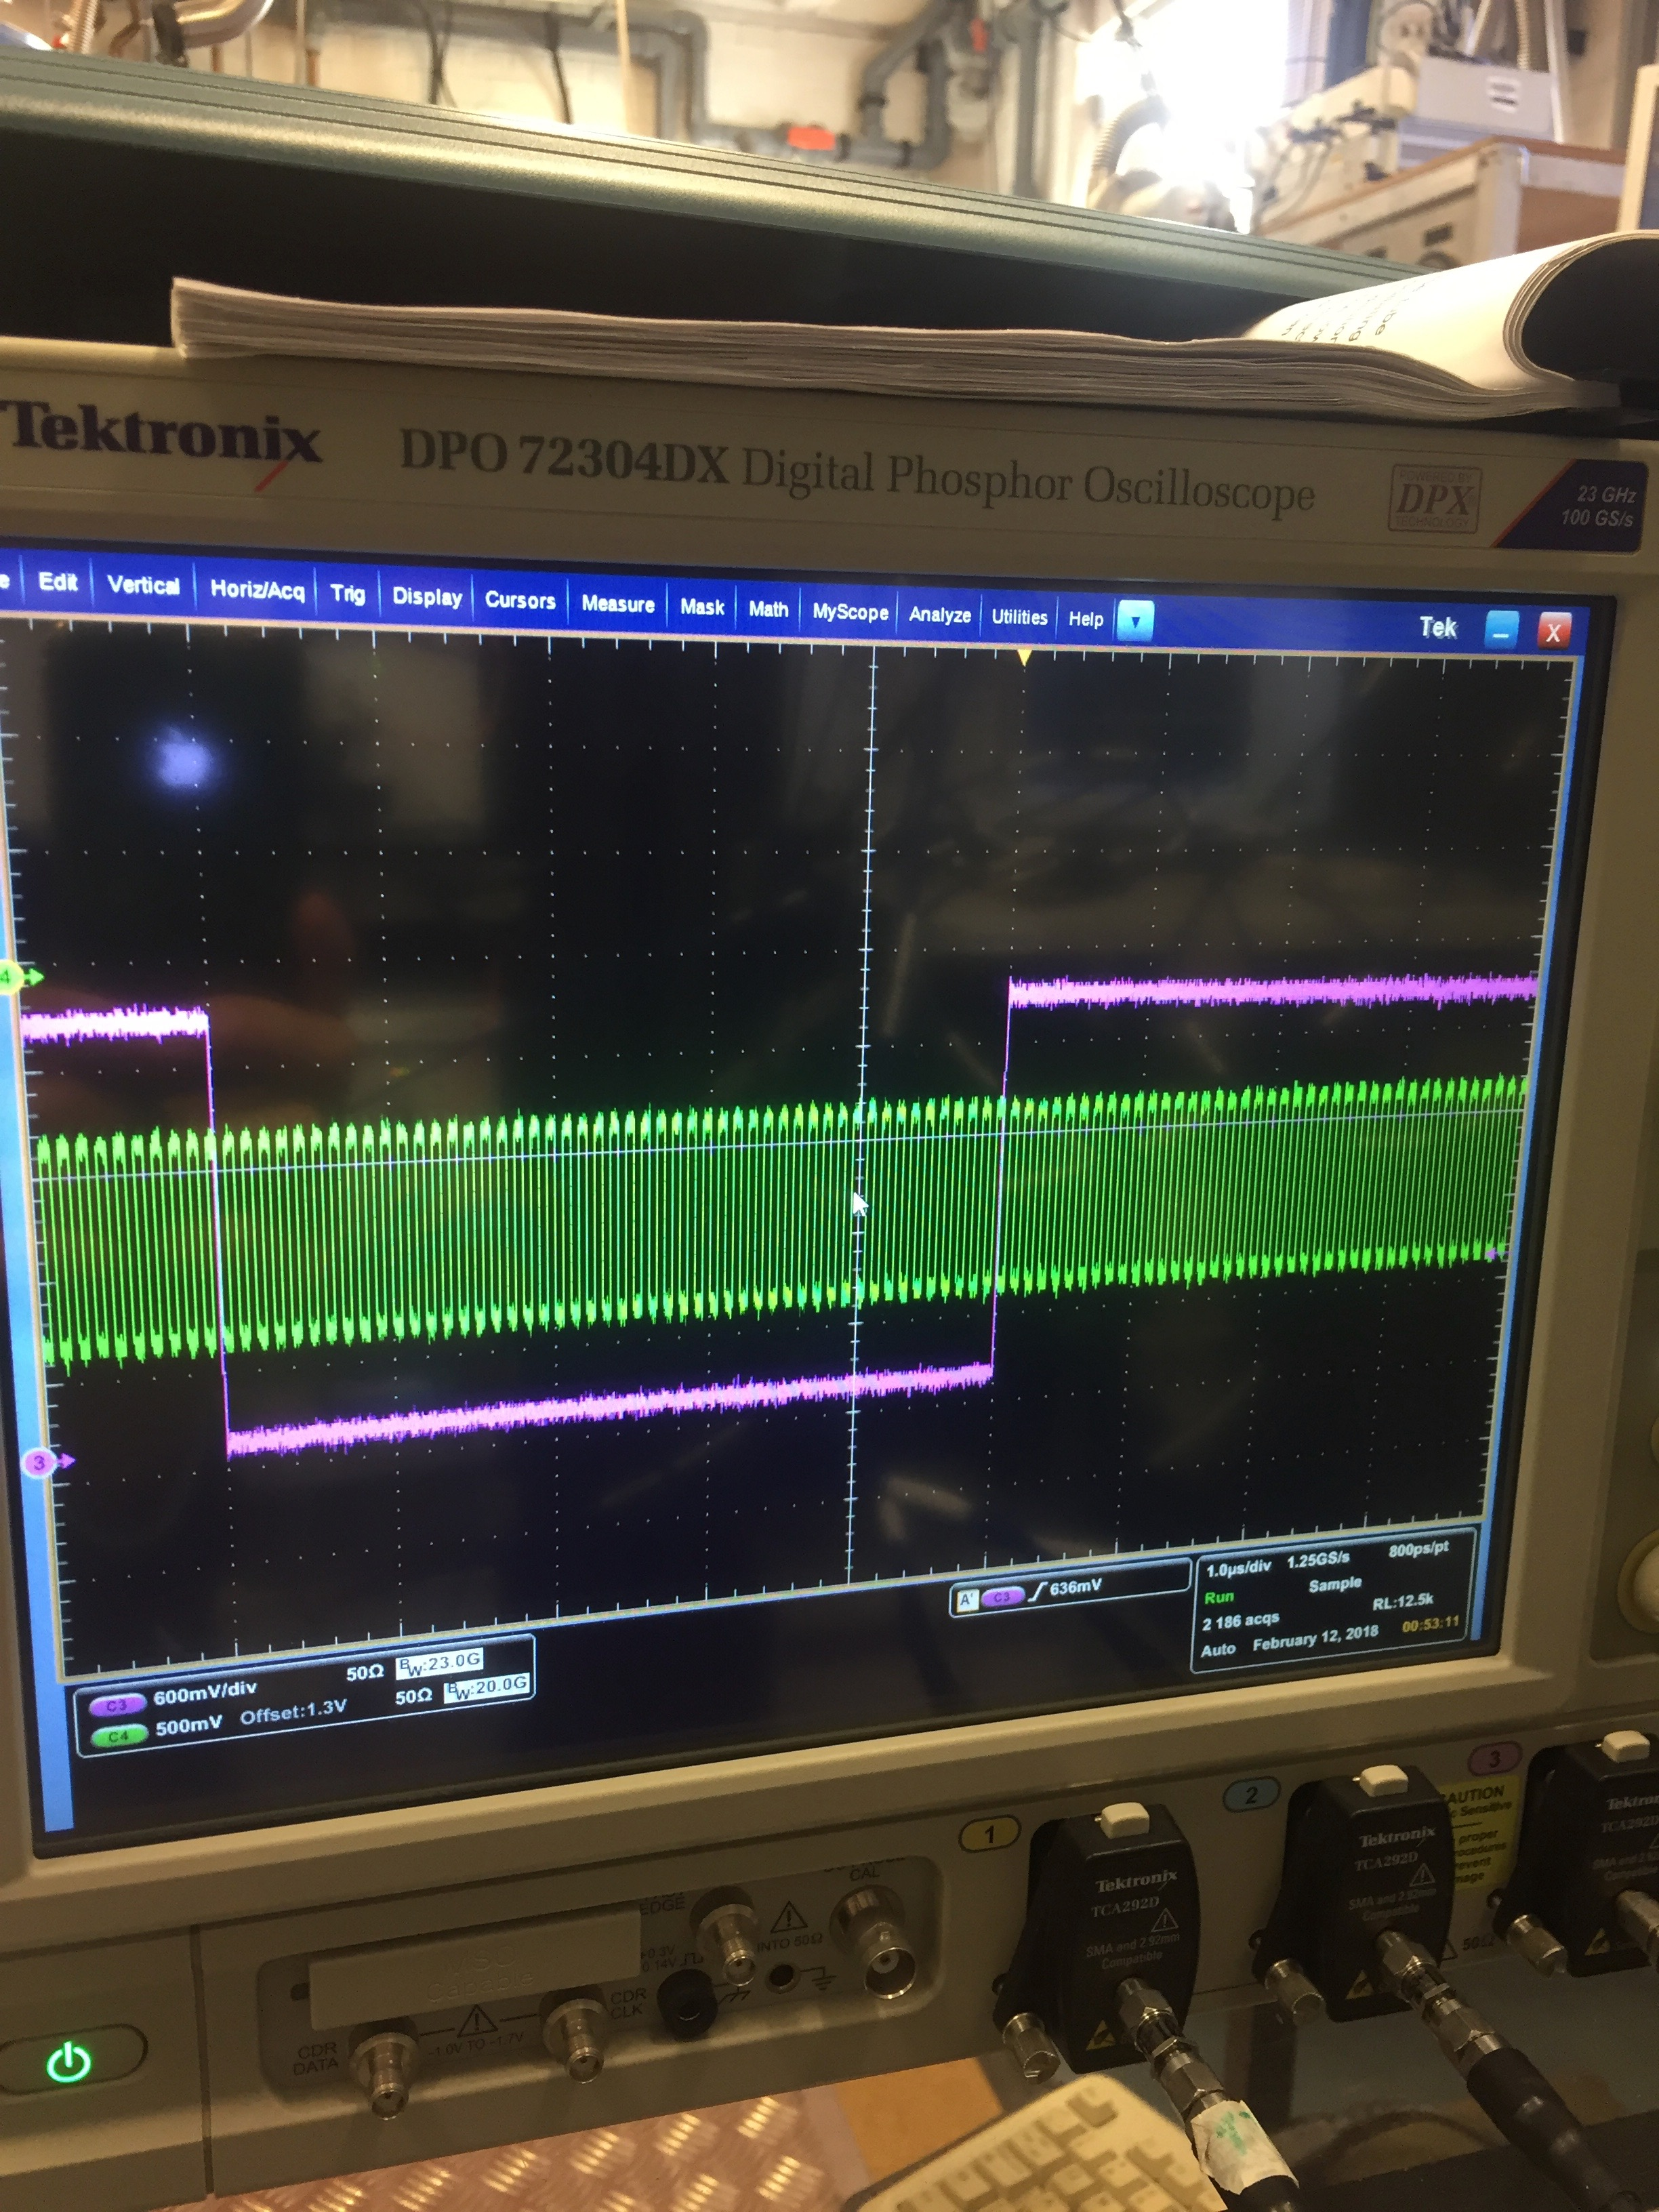
\includegraphics[height=2cm]{sync1}
		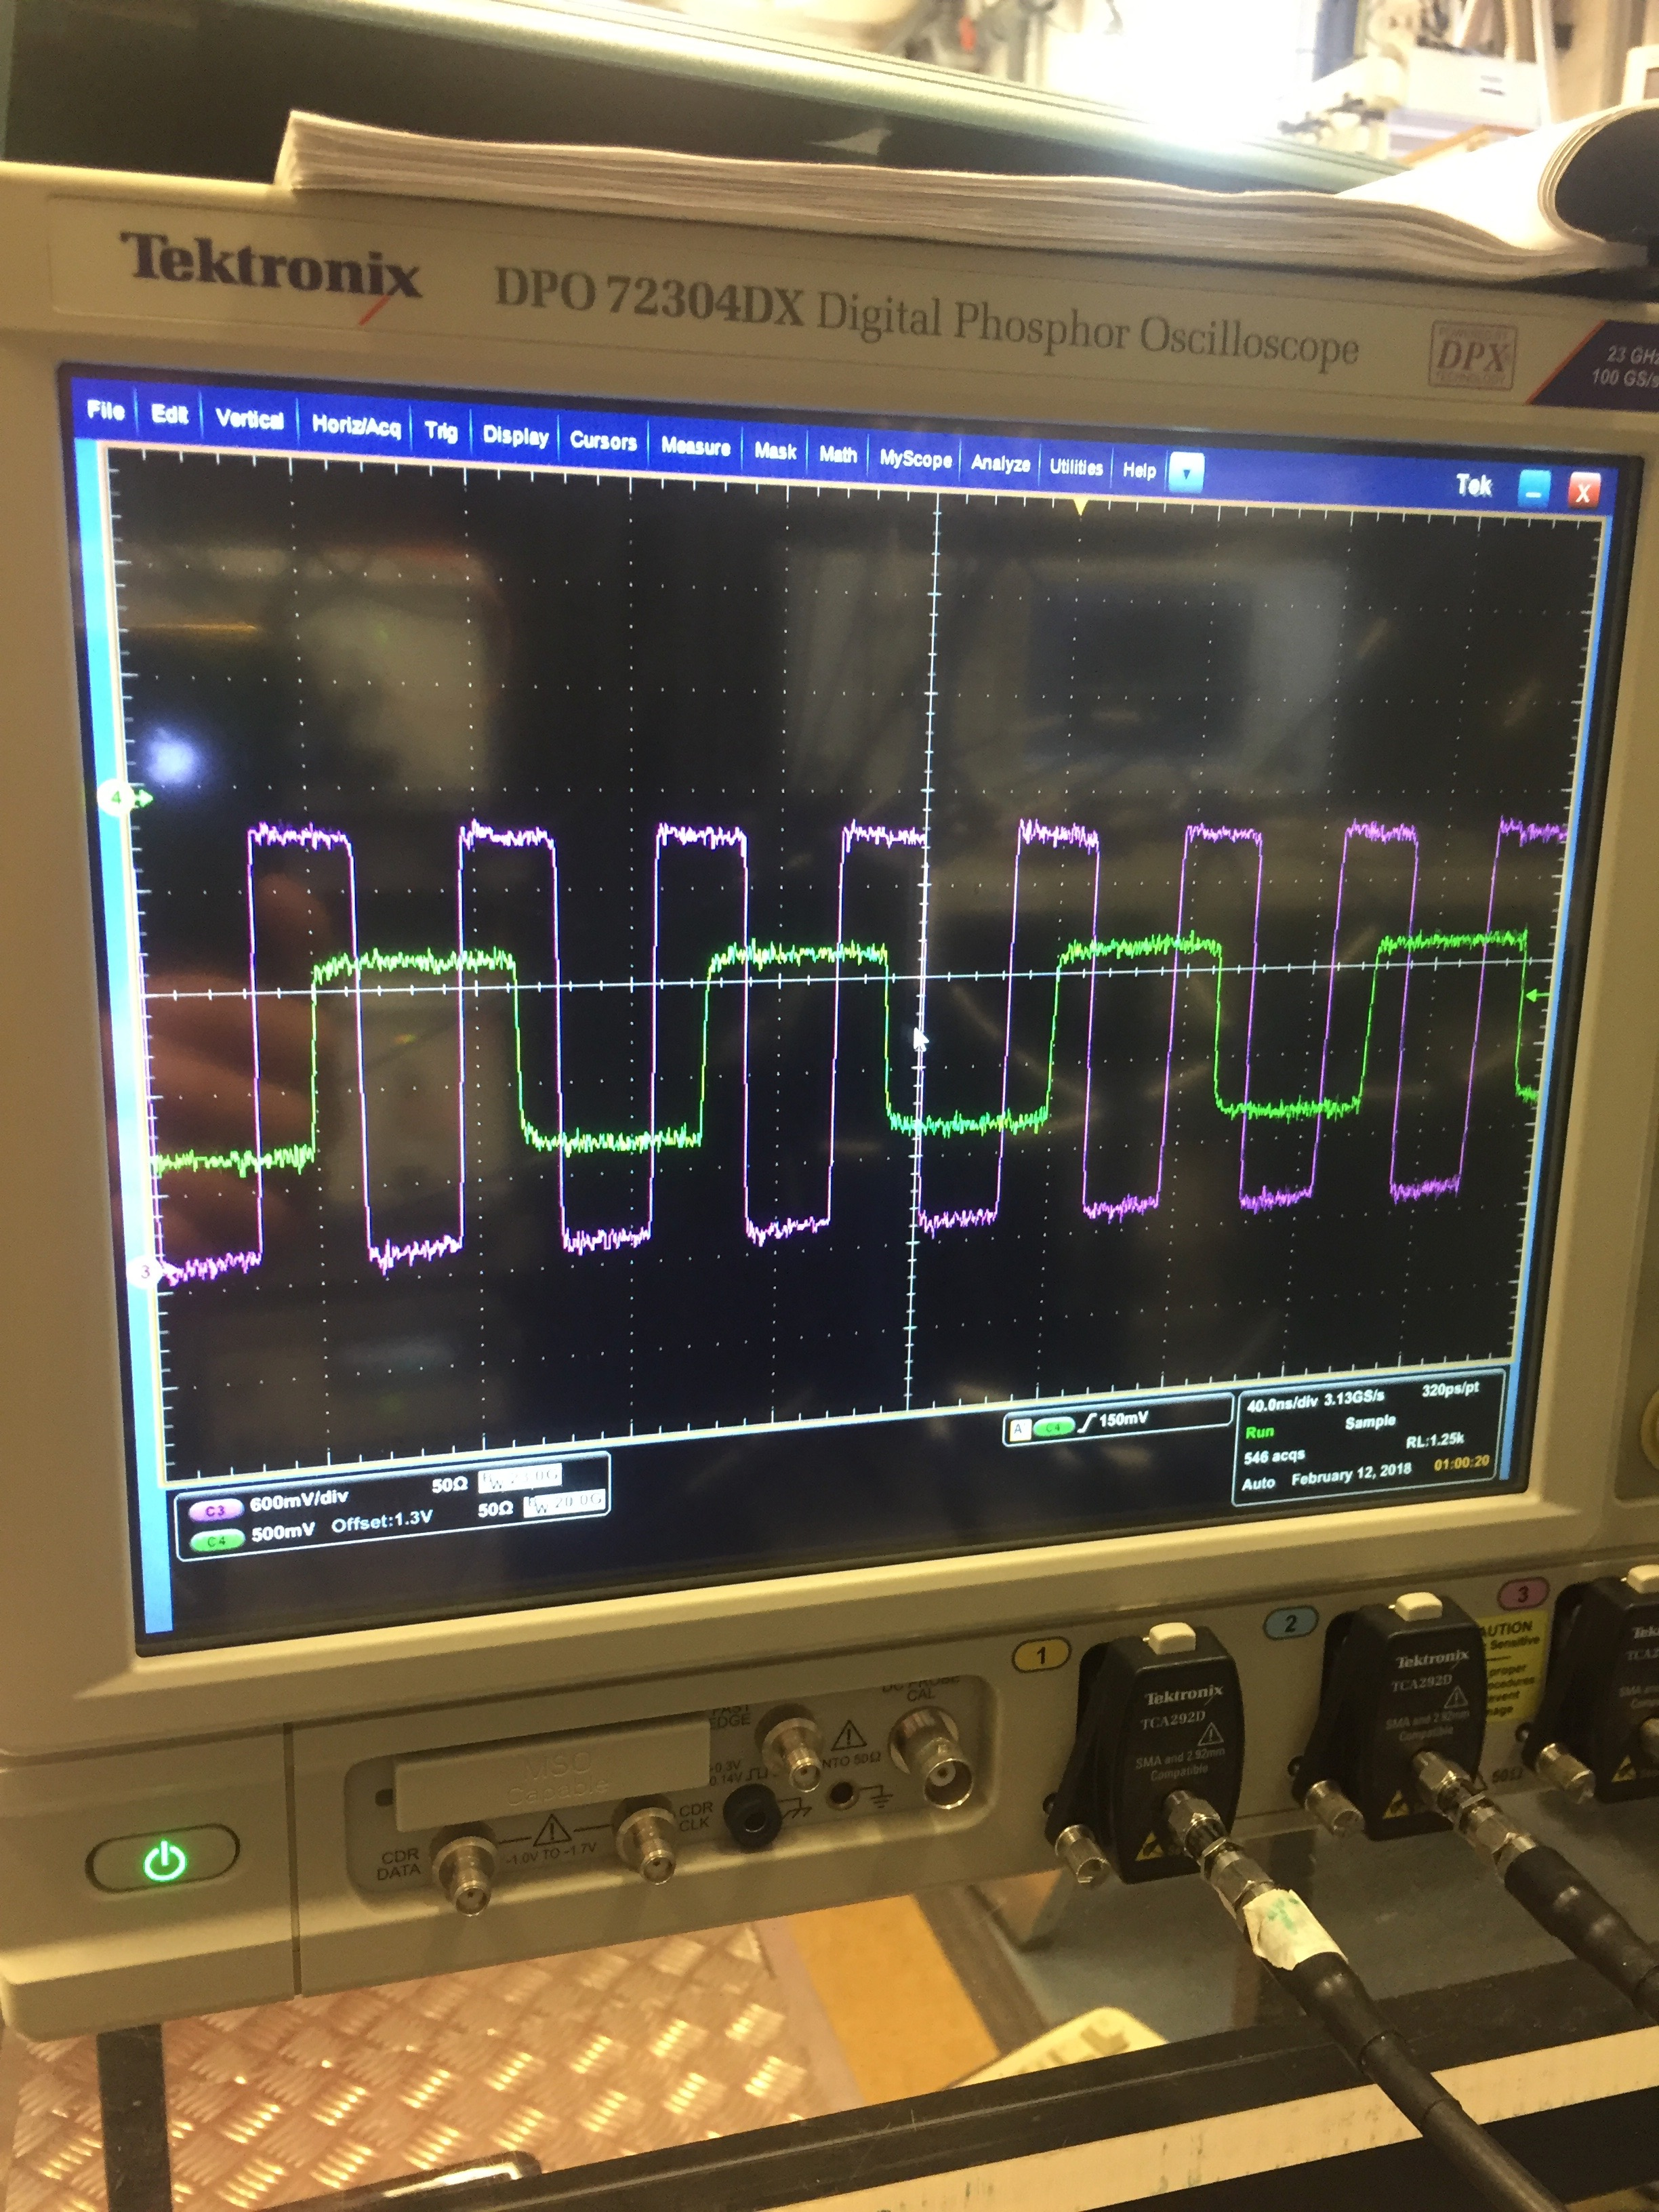
\includegraphics[height=2cm]{sync2}
		\caption{The two images, in which green is the 10\,MHz clock signal, and pink is the 10\,kHz or 20MHz pulse signal. The picture is stationary, meaning that they are in sync.}
	\end{figure}
 
 \newpage
 